% Replacement pages 3--5 for the group-meeting note.
% The merge script physically prepends unchanged source pages 1--2.
\documentclass[11pt]{article}
\usepackage[letterpaper,margin=1.72cm]{geometry}
\usepackage{amsmath,amssymb}
\usepackage{booktabs,array,tabularx,colortbl}
\usepackage{graphicx,xcolor}
\usepackage{float,enumitem,microtype}
\usepackage[font=small,skip=3pt]{caption}
\usepackage{titlesec}
\titlespacing*{\section}{0pt}{2pt}{4pt}
\setlength{\abovedisplayskip}{4pt}
\setlength{\belowdisplayskip}{4pt}
\setlength{\textfloatsep}{5pt}
\setlist[itemize]{leftmargin=*,topsep=2pt,itemsep=2pt,parsep=0pt}
\newcolumntype{L}[1]{>{\raggedright\arraybackslash}p{#1}}
\newcolumntype{Y}{>{\raggedright\arraybackslash}X}
\definecolor{incpurple}{HTML}{7E57A6}
\definecolor{arrivalgreen}{HTML}{008A65}
\definecolor{searchblue}{HTML}{1769AA}
\definecolor{softpurple}{HTML}{F2EAF7}
\definecolor{softgreen}{HTML}{E8F5EF}
\definecolor{softblue}{HTML}{EAF3FA}
\newcommand{\takeaway}[1]{\par\smallskip\noindent\textbf{Takeaway.} #1\par\smallskip}
\newcommand{\regI}{\mathrm I}
\newcommand{\regA}{\mathrm A}
\newcommand{\regE}{\mathrm E}
\newcommand{\WPBE}{\mathrm{WPBE}}

\begin{document}
\setcounter{page}{3}
\setcounter{section}{1}

\section{Three new directions share one nested WPBE design}

\takeaway{Starting from the two-page benchmark, we change only second-window
supply: retained incumbents, time-homogeneous fresh arrivals, and finally an
expanded rescue footprint.  Prices and search are always optimized outside the
induced cutoff-WPBE.}

\begin{center}
\small
\renewcommand{\arraystretch}{1.18}
\begin{tabularx}{.99\textwidth}{@{}L{2.05cm}L{2.25cm}Y L{2.35cm}@{}}
\toprule
Architecture & Policy & Who can volunteer in window 2 & What it identifies\\
\midrule
\rowcolor{softpurple}
\textcolor{incpurple}{\textbf{$\regI$: retained incumbents}} & $(p_1,p_2)$ & First-window rejectors who remain available & Same-order recall value\\
\rowcolor{softgreen}
\textcolor{arrivalgreen}{\textbf{$\regA$: fixed footprint + arrivals}} & $(p_1,p_2)$ & Retained rejectors plus an independent fresh core cohort & Time-homogeneous replenishment\\
\rowcolor{softblue}
\textcolor{searchblue}{\textbf{$\regE$: expanded rescue search}} & $(p_1,p_2,s)$ & The same core supply plus an outer annulus reached only in rescue & Incremental geographic reach\\
\bottomrule
\end{tabularx}
\end{center}

Here $p_j$ is one anonymous transaction price: the rider pays $p_j$ and the
assigned driver receives $p_j$.  The local per-window flows are
\[
N_1\sim\operatorname{Pois}(m),\qquad
N_2^C\sim\operatorname{Pois}(m),\qquad
N_2^O(s)\sim\operatorname{Pois}(m(s-1)).
\tag{5}
\]
Conditional on first-window cutoff $a$, define retained-incumbent, fresh-core,
and outer-annulus volunteer intensities by
\[
 I_j(a)=\omega m[F(p_j)-F(a)]_+,\quad
 E_j^C=mF(p_j),\quad
 E_2^O(s)=m\!\int_1^s F\!\left(p_2-\tau(\sqrt u-1)\right)du.       \tag{6}
\]
The total terminal intensity is
\[
 \lambda_j^r(a)=I_j(a)+\mathbf 1\{r\ne\regI\}E_j^C
 +\mathbf 1\{r=\regE,j=2\}E_2^O(s),\quad
 C_j^r=1-e^{-\lambda_j^r},\quad h(\lambda)=\frac{1-e^{-\lambda}}{\lambda}.
\tag{7}
\]
Thus every $\lambda$ is an expected Poisson volunteer count, $C$ is coverage,
and $h$ is one volunteer's lottery win probability.  Only
$\regA\subset\regE$: $s=1$ reproduces the fixed footprint, while the rescue
radius is $R_0\sqrt{s}$.

\begin{minipage}[t]{.445\textwidth}
\vspace{0pt}\raggedright
\textbf{Information and incentives.}
Incumbents have seen the order and commitment, so they may reject and wait.
Fresh drivers first see it in window 2.  Universal rejection is public; the
rider observes failure but not realized counts, and uses equilibrium coverage.
A rejector remains eligible with probability $\omega$.
\end{minipage}\hfill
\begin{minipage}[t]{.445\textwidth}
\vspace{0pt}\raggedright
\textbf{Two different costs.}
An assigned outer driver pays the post-assignment pickup cost embedded in
(6).  Separately, after failure the platform reserves capacity for its promised
outer footprint:
\[
Q^{\mathrm{com}}=(1-p_1)e^{-ma}m(s-1).
\tag{8}
\]
Thus free search is not built into the objective.
\end{minipage}

\medskip
Every plotted policy is evaluated at its own cutoff-WPBE:
\[
V_r(\theta)=\max_{\mu_r}\ J_r\bigl(\mu_r,a^*(\mu_r;\theta)\bigr),
\quad J_r=M_r-\kappa Q_r^{\mathrm{com}},
\quad
\boxed{\text{fix }p_1\ \to\ \max_{p_2,s}\ \to\ \max_{p_1}}.
\tag{9}
\]
The inner cutoff $a^*$, rider continuation, and supply composition are all
re-solved at every outer-policy evaluation; $s$ is present only for $\regE$.

\clearpage
\section{Directions 1--2: isolate the value of fresh arrivals}

\takeaway{Adding a fresh core cohort has its largest displayed value in a
moderately thick market; the option to search outside the core is most valuable
earlier, when the local market is still thin.}

\begin{figure}[H]
\centering
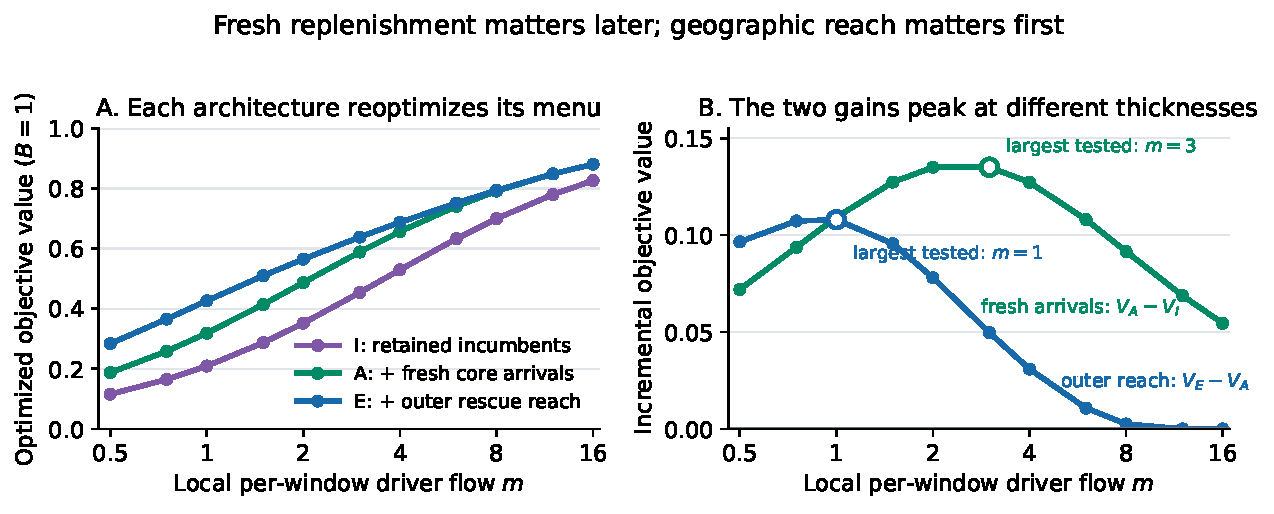
\includegraphics[width=.995\textwidth]{../figures/figure_reoptimized_values.pdf}
\caption{Illustrative slice
$(\beta,\delta,\omega,\tau,\kappa,\bar s)=(.8,.8,.8,.25,.0125,4)$ with
$v,c\sim U[0,1]$ and $B=1$.  Every point separately reoptimizes all controls
available to that architecture and re-solves the cutoff-WPBE.  $\regI$ and
$\regA$ report completion; $\regE$ reports completion net of committed-reach
cost.}
\end{figure}

\begin{itemize}
\item \textcolor{arrivalgreen}{\textbf{$\regI\to\regA$: replenishment.}}
Fresh arrivals directly raise second-window coverage and also compete with
rejectors who wait.  The gain is therefore an equilibrium response, not a
fixed-policy supply addition.
\item \textcolor{searchblue}{\textbf{$\regA\to\regE$: reach option.}}
Because $s=1$ is feasible, this net option value is nonnegative.  Its largest
tested value occurs around $m=1$, before the fresh-core value reaches its
largest tested value around $m=3$.
\item \textbf{Interpret the peaks cautiously.}  The plot supports two distinct
economic regions and an ordered-peak conjecture; it does not claim unique
global peaks in the fully endogenous WPBE model.
\end{itemize}

\clearpage
\section{Direction 3: expanded search is an early-thickness tool}

\takeaway{Market thickness changes the mix of recovery tools.  Search scope
contracts sharply with $m$, but a positive rescue price increment remains even
after the optimized footprint returns to the core.}

\begin{figure}[H]
\centering
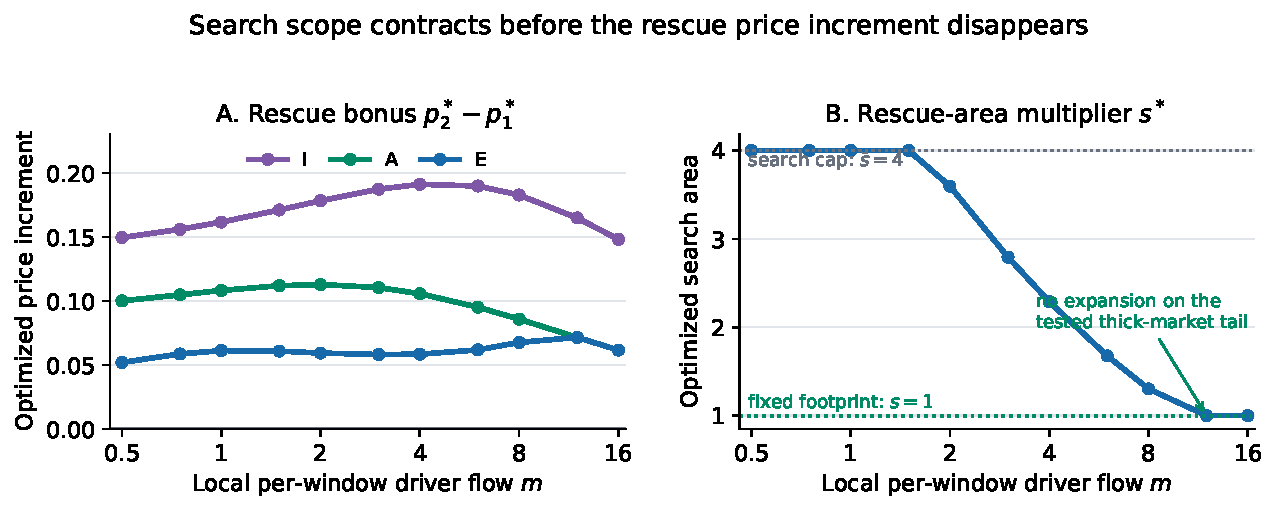
\includegraphics[width=.995\textwidth]{../figures/figure_optimal_controls.pdf}
\caption{Same calibration and equilibrium-constrained optimization as page 4.
The right panel uses committed-reach cost; $s=1$ means no expansion beyond the
fresh core cohort.}
\end{figure}

\begin{center}
\small
\renewcommand{\arraystretch}{1.14}
\begin{tabularx}{.97\textwidth}{@{}L{2.0cm}Y Y@{}}
\toprule
Market region & Main shortage & Numerical mechanism intuition\\
\midrule
Thin & Too few reachable drivers & Expand aggressively; the tested optimum reaches the search cap.\\
Intermediate & Coverage and strategic waiting both matter & Combine a rescue increment with a gradually shrinking outer footprint.\\
Thick & The core is already reliable & Set $s=1$ on the tested tail, while retaining a positive $p_2-p_1$.\\
\bottomrule
\end{tabularx}
\end{center}

\medskip
\noindent\colorbox{softblue}{\parbox{.965\textwidth}{\small
\textbf{Current story.}  Fresh arrivals and expanded search are different
sources of recovery value.  Search is an early-thickness tool; rescue pricing
continues to manage screening and delayed acceptance after geographic expansion
is no longer worth its capacity cost.}}

\medskip
The next theory step is deliberately deferred: primitive conditions for peak
ordering and the exact no-search threshold in $\kappa$.  The complete theory
note keeps those claims, proofs, counterexamples, and literature boundaries
separate from this five-page intuition-and-simulation presentation.

\end{document}
